\documentclass{lkx_paper}

\title{\textbf{Compact Riemann Surfaces of Genus 1}}
\date{}
\author{Lev Kruglyak}

\usepackage{graphicx}

\newcommand{\D}{\mathbb{D}}
\newcommand{\x}{\mathbf{x}}
\usepackage{pgfplots}
\pgfplotsset{
	compat=1.12,
}


\begin{document}
\maketitle

\tableofcontents

\section{Introduction}

Riemann surfaces were originally studied as in the 19th centry in the context of complex analysis. As they are complex manifolds of one dimension, they serve as the natural habitat for the investigation of complex function in a single variable. Riemann's revolutionary idea was that many multivalued complex functions are better understood as maps between Riemann surfaces as opposed to maps from the complex plane.

The study of these surfaces has grown into a well-understood and pivotal area of mathematics that lies at the intersection of complex analysis, topology, and algebraic geometry. In this paper, we'll discuss compact Riemann surfaces of genus 1, which turn out to be topological tori with additional complex geometric structure. In particular, these Riemann surfaces turn out to have deep relationships to lattices in the plane and to the theory of elliptic functions.

Moreover, the history of these surfaces is rich with mathematical innovation. The exploration of elliptic functions, initially motivated by the need to invert elliptic integrals arising in physics and astronomy, led to significant advancements in the theory of functions and complex analysis. We'll begin our journey with the classical problem of predicting the motion of the planets in the night sky. The study of the orbits of the planets led mathematicians to discover elliptic integrals, and from there elliptic functions which tie in naturally to our story.

\subsection{Elliptic Integrals}

With Newton's law of gravitation, we can find explicit formulas to predict the motion of the planets in the sky. Suppose we have two planetary bodies of masses $M$ and $m$ respectively, and fix a frame of reference to the larger body with mass $M$. The total energy of this system is then
\[
	E = \frac{mv^2}{2} - \frac{GMm}{r}
\]
where the smaller body moves with velocity $v$ at distance $r$ to the larger body.
Rewriting $v$ in polar coordinates as $(r_v, \theta_v)$, we get $v^2 = r_v^2 + r^2\theta_v^2$. Then by a series of clever substitutions and applying principles of Newtonian physics, we find that
\[
	\theta = \textrm{arccos}\left(\frac{1/r - 1/a}{e/a}\right),\quad\textrm{and}\quad r=\frac{a}{1+e\cos\theta},
\]
where $a$ and $e$ are defined
\[
	a=\frac{L^2}{GMm^2},\quad e=\sqrt{1+\frac{2Ea}{GMm}}\quad\textrm{for } L=r\times mv\textrm{ the angular momentum.}
\]
In other words, the path traced out by the smaller body is an ellipse with one focus at the origin. This gives us a justification of Newton's laws from the observed principles of Kepler, but we get even more. Since we know that an ellipsed is parametrized by $(a\cos t, b\sin t)$, a common calculation might be to evaluate the integral
\[
	\int_{t_0}^{t_1} \sqrt{a^2\sin^2 t + b^2\cos^2 t}\,dt
\]
which represents the distance covered by the smaller body in a given time interval. For a simpler expression, we might rewrite this integral as
\[
	\int_{t_0}^{t_1} \sqrt{a^2\sin^2 t + b^2\cos^2 t}\,dt = b\int_{\sin t_0}^{\sin t_1} \frac{\sqrt{1-k^2x^2}}{\sqrt{1-x^2}}\,dx\quad\textrm{for}\quad k = 1 - \left(\frac{a}{b}\right)^2.
\]
Such integrals came to be known as \emph{elliptic integrals}, and quickly became objects of study by mathematicians. These functions were particularly tricky because most of the time, these integrals have no closed form expression in terms of elementary functions.
\begin{definition}
	An \defn{elliptic integral} is a function $f$ which can be expressed in the form
	\[
		f(x) = \int_c^x R(t, \sqrt{P(t)})\,dt,
	\]
	where $R$ is a rationaal function, and $P$ is a polynomial of degree $3$ or $4$ with no repeated roots, and $c$ is a constant.
\end{definition}

\subsection{Elliptic Functions}
The general theory of elliptic integrals is deep and complicated, however we might notice a familiar pattern from our studies of complex analysis. Recall that have formulas
\[
	\log(z) = \int \frac{dz}{z}\quad\textrm{and}\quad \sin^{-1}(z) = \int\frac{dz}{\sqrt{1-z^2}}.
\]
In both of these cases, the inverse of a periodic function ($\exp$ and $\sin$) respectively can be expressed as the integral of a reciprocal. In the former case, $\log(z)$ conformally maps the upper half-plane $\mathbb{H}$ to a bigon with external angles of $\pi$, i.e. the strips $0<\textrm{Im } z<\pi$, and the latter maps the upper half plane $\mathbb{H}$ to a triangle defined by $\textrm{Im } z > 0$, $|\textrm{Re }z| < \pi/2$. This pattern is generalized by the \emph{Schwarz-Christoffel formula}, which provides an explicit formula for the Riemann mapping to a polygonal region.

\begin{theorem}[Schwarz-Christoffel Formula]
	Let $f : \mathbb{H} \to U$ be the Riemann mapping to a polygon with vertices $\{p_i\}_{i=1}^n$ and exterior angles $\{\pi \mu_i\}_{i=1}^n$. Then, we have
	\[
		f(\zeta) = \alpha\int \frac{d\zeta}{\prod_{i=1}^n (\zeta-q_i)^{\mu_i}}+\beta,
	\]
	where $f(q_i)=p_i$.
\end{theorem}

From this, we see that if $P(t)$ is a quadratic polynomial, then
\[
	f(\zeta) = \int \frac{d\zeta}{\sqrt{P(\zeta)}}
	=\int \frac{d\zeta}{(\zeta-q_1)^{1/2}(\zeta-q_2)^{1/2}(\zeta-q_3)^{1/2}(\zeta-q_4)^{1/2}}
\]
is a Riemann mapping of the upper half-plane to a square in $\C$, under some appropriate conditions on $f(q_i)$. Inverting $f$, we get a function from a square to $\mathbb{H}$. If we tile the entire complex plane by $f$ using Schwarz reflection, we get what's called an \emph{elliptic function}.

\begin{definition}
	Let $\Lambda\subset \C$ be a lattice, say with $\Lambda = \alpha\Z\oplus \beta\Z$ for some basis $\alpha,\beta\in \C$. An \defn{elliptic function} is some meromorphic function $f : \C \to \widehat{\C}$ with
	\[
		f(z + \alpha)=f(z)\quad\textrm{and}\quad f(z+\beta)=f(z).
	\]
	Equivalently, an elliptic function is a meromorphic function $f : E \to \widehat{\C}$ where $E=\C/\Lambda$ is the complex torus associated to the lattice.
\end{definition}

These functions form a field, which we call $\mathcal{M}(E)$.

\subsection{The Weierstrass \texorpdfstring{$\wp\,$}{p}-function}

By Liouville's theorem, any holomorphic elliptic function must be constant because the fundamental parallelogram of the lattice is compact. Thus, to find some explicit form for an elliptic function, we must allow for poles. We might try the functions
\[
	\zeta_k(z) = \sum_{\lambda\in \Lambda}\frac{1}{(z-\lambda)^k},
\]
however these only converge for $k\geq 3$. To get the series to converge for $k=2$, we make a modification by a constant factor in each term of the sum.

\begin{definition}
	For a lattice $\Lambda\subset \C$, the \defn{Weierstrass $\wp$-function} is given by
	\[
		\wp(z) = \frac{1}{z^2} + \sum_{\lambda\in \Lambda\setminus\{0\}} \frac{1}{(z-\lambda)^2} - \frac{1}{\lambda^2}.
	\]
\end{definition}

This is an even meromorphic function on the compact Riemann surface $E$, and it has a unique pole of order $2$ on $E$.

\begin{proposition}
	The Wierstrass $\wp$-function is elliptic.
\end{proposition}
\begin{proof}
	Since $\wp'(z)=-2\zeta_3(z)$, it is an elliptic function so $\wp(z+a)=\wp(z)+A$ and $\wp(z+b)=\wp(z)+B$ for some constants $A$ and $B$. But $\wp(-z)=\wp(z)$, so if we set $z=a/2$ and $b/2$ respectively, we get that $A=0$ and $B=0$.
\end{proof}

\begin{figure}[ht]
	\centering
	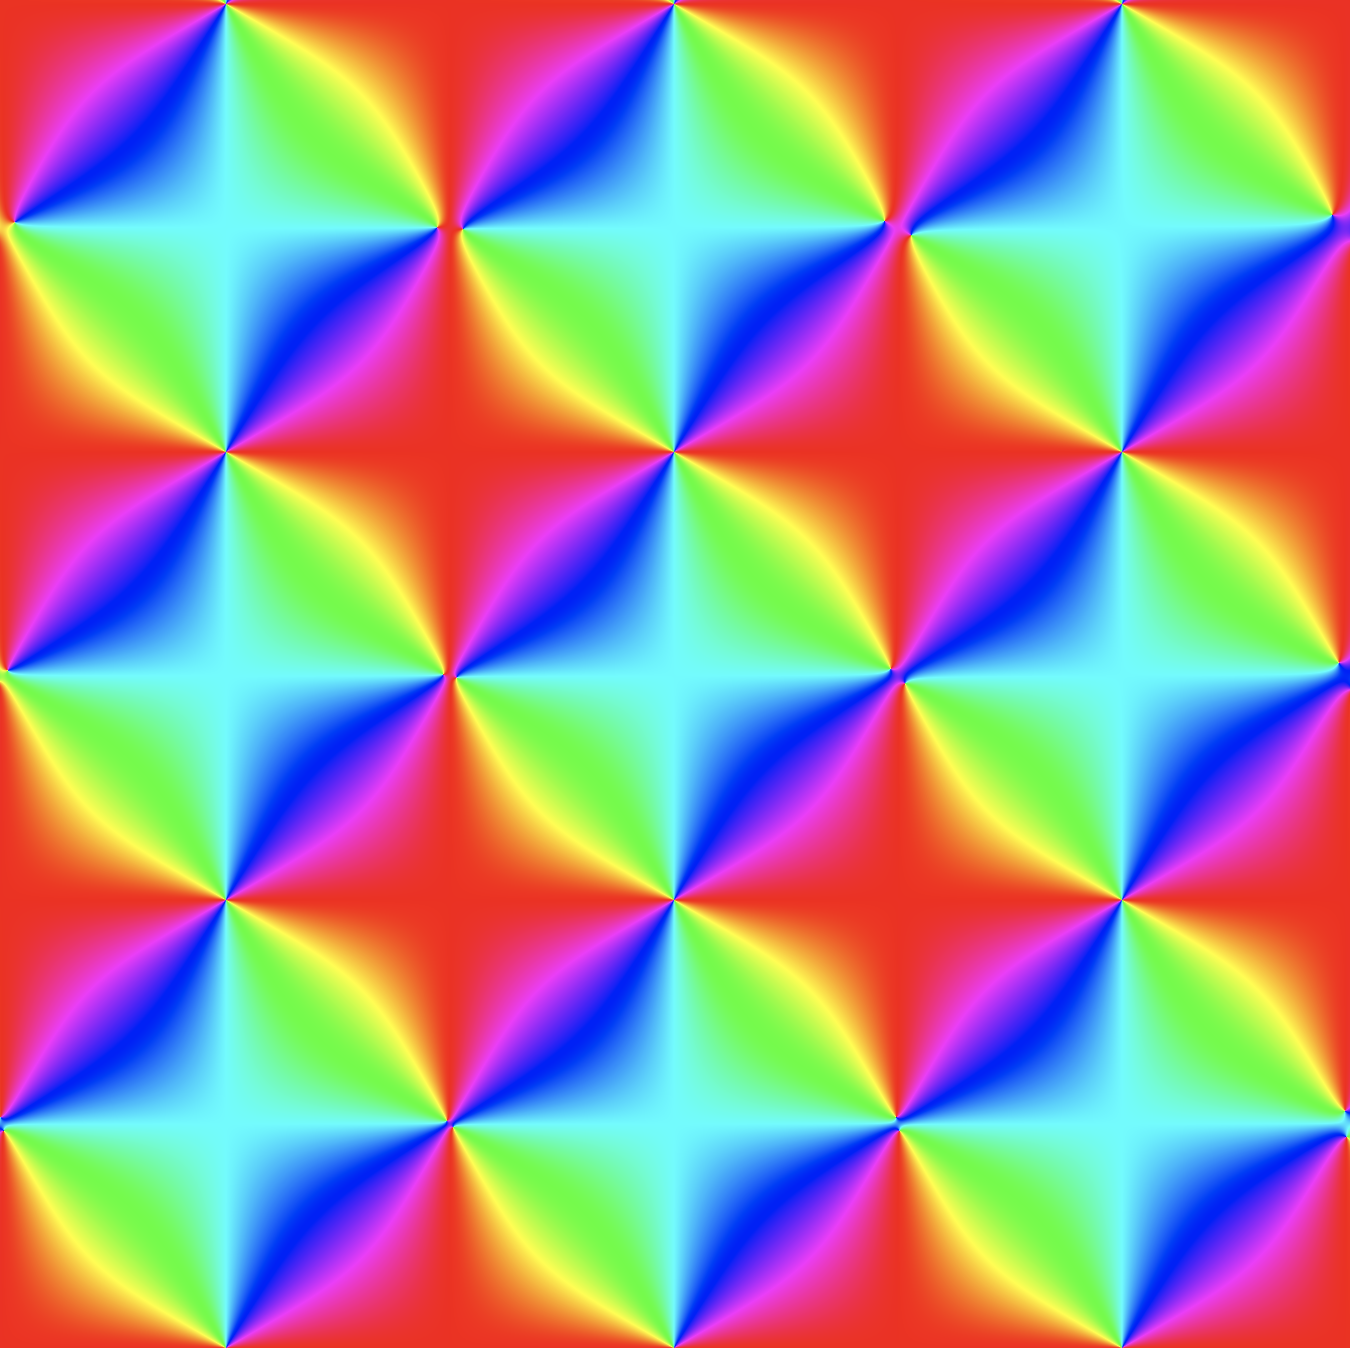
\includegraphics[scale=0.25]{pfunction_square.png}
	\hspace{0.5in}
	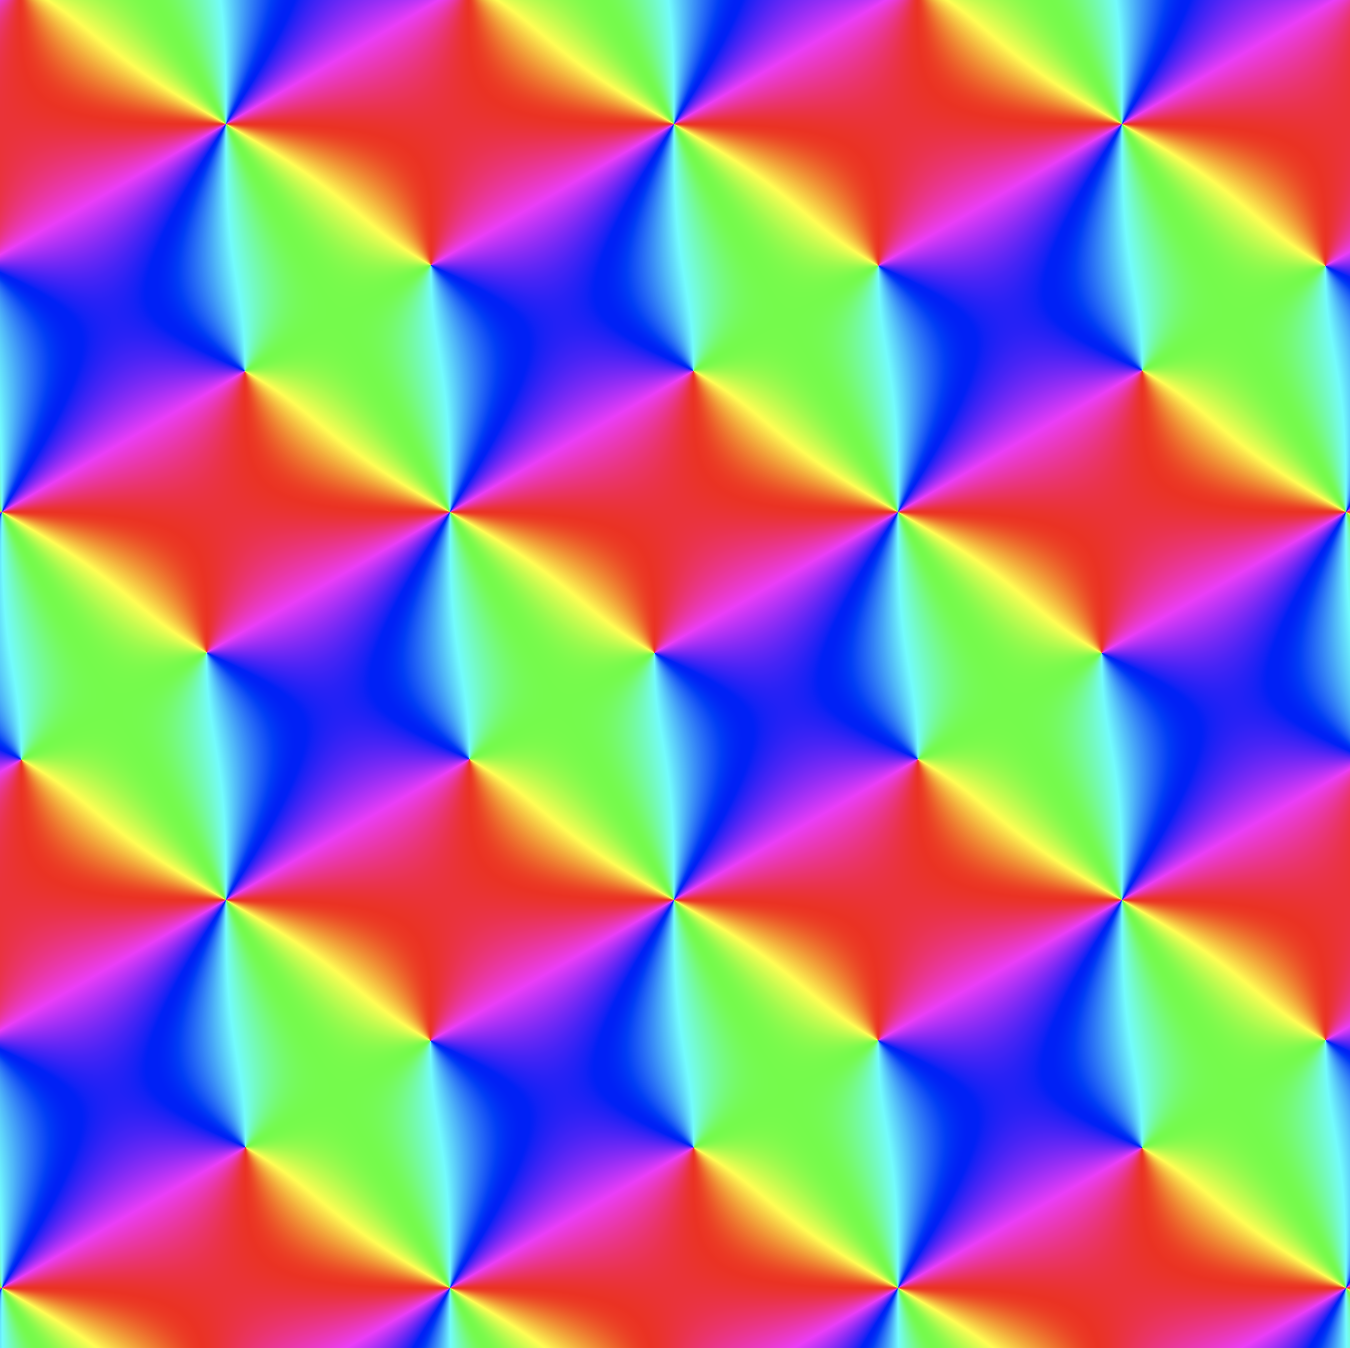
\includegraphics[scale=0.25]{pfunction_hex.png}
	\caption{Domain colored graphs of the Weierstrass $\wp$-function for the square and hexagonal lattices respectively.}
\end{figure}

\section{Elliptic Curves}
Exploring the Weierstrass $\wp$-function in more detail, we see that it has derivative
\[
	\wp'(z) = -2\sum_{\lambda\in \Lambda} \frac{1}{(z-\lambda)^3} = -2\zeta_3(z).
\]
This is an odd elliptic function. With some manipulation of the series involved, we obtain a fundamental differential equation at the heart of elliptic function theory.
Let's define the \emph{holomorphic Eisenstein series of weight }$2k$ as the infinite series
\[
	G_{2k}(\tau) = \sum_{(m,n)\in \Z^2\setminus \{(0,0)\}}\frac{1}{(m+n\tau)^{2k}}
\]
for $\tau \in \mathbb{H}$. From now on, we'll scale our lattice so that $\Lambda = \Z\oplus \tau\Z$.
\begin{theorem}
	We have the differential equation:
	\[
		\wp'(z)^2 = 4\wp(z)^3 - g_2 \wp(z) -g_3,
	\]
	where $g_2 = 60 G_4(\tau)$ and $g_3=140 G_6(\tau)$.
\end{theorem}

This is an example of an elliptic curve! Recall the definition of an elliptic curve:

\begin{definition}
	An \defn{elliptic curve} over a field $k$ is a smooth, projective algebraic curve of genus one with specified basepoint. It can be described as an algebraic curve consisting of solutions
	\[
		y^2 = x^3+ax+b,
	\]
	for coefficients $a,b\in k$, under the condition that it is non-singular, or that $4a^3+27b^2\neq 0$.
\end{definition}

These quantities $g_2$ and $g_3$ are fundamental invariants of the lattice $\Lambda$, and turn out to perfectly classify lattices under \emph{homothety}, or scaling the lattice by a constant factor.

A natural consequence of this differential equation is the following theorem:
\begin{theorem}
	The map $\pi : \C \to \CP^2$ given by
	\[
		\pi(z) = \begin{cases}
			[\wp(z) : \wp'(z) : 1] & z\in \C\setminus\Lambda , \\
			[0 : 1 : 0]            & z \in \Lambda,
		\end{cases}
	\]
	descends to an isomorphism between $E$ and the smooth projective cubic curve of the form $y^2z=4x^3+axz^2+bz^3$, which is the homogenized version of the elliptic curve equation.
\end{theorem}
It's a deep fact in the study of Riemann surfaces that every compact Riemann surface is embeddable in the complex projective plane as an algebraic curve, but here we have an explicit such embedding for the case of complex curves!

Even more remarkably, the Weierstrass function and its derivative are the \emph{only} elliptic functions needed to construct all of the others. In other words,
\begin{theorem}
	The field of elliptic functions for a given lattice, i.e. $\mathcal{M}(\C/\Lambda)$ satisfies
	\[
		\mathcal{M}(\C/\Lambda) \cong \frac{\C[x,y]}{y^2-(4x^3+g_2x+g_3)}.
	\]
\end{theorem}

\section{Compact Riemann Surfaces of Genus 1}

So far, we've exhibited the following connection:
\[
	\left\{\begin{array}{c}\textrm{elliptic curves}\\ \textrm{over } \C\end{array}\right\}
	\quad\iff\quad \left\{\begin{array}{c}
		\textrm{lattices }\Lambda\subset \C \\\textrm{up to homothety}
	\end{array}\right\}.
	\quad\iff\quad \left\{\begin{array}{c}
		\textrm{Riemann surfaces} \\\textrm{of the form }\C/\Lambda
	\end{array}\right\}
\]
The next question we might ask is if we found all of the compact Riemann surfaces of genus 1 or if there are any others. If there aren't, then we've completely classified this class of surfaces, connecting them to lattices, and exhibiting them as projective algebraic curves. To understand this better, we must go a bit deeper into the theory of Riemann surfaces.

\subsection{Poisson Equation}

Yet another fundamental equation coming from physics is the Poisson equation, a partial differential equation which takes the classical form
\[
	\left(\frac{\partial^2}{\partial x_1^2}+\cdots + \frac{\partial^2}{\partial x_n^2}\right)\psi = \rho.
\]
When $\rho=0$, solutions to this equation are called \emph{harmonic functions}. This equation shows up in the theory of gravitation, fluid dynamics, electrostatics, spherical harmonics, and many other fields. It also turns out to have deep utility in the theory of Riemann surfaces under a suitable generalization.

Let $X$ be a compact connected Riemann surface, and let $\rho\in \Omega^2(X)$ be an area form which satisfies $\int_X \rho = 0$. Let $\Delta$ be the Laplace-Beltrami operator, given by $\Delta = \star d\star d$.

\begin{definition}
	The \defn{Poisson equation} states that $\Delta \varphi = \rho$ for some $\varphi\in \Omega^0(X)$.
\end{definition}

\begin{theorem}[Fundamental Theorem]
	There is a solution to the Poisson equation, unique up to the addition of a constant.
\end{theorem}
\begin{proof}
	We defer this proof to Section~9 of \cite{donaldson}.
\end{proof}

This theorem has important ramifications in the differential topology of Riemann surfaces, and complex manifolds in general.

\subsection{Dolbeault Cohomology}

In the complex setting, ordinary de Rham cohomology is insufficient to describe the full richness of complex differential forms. Here, we decompose the differentials of standard coordinates $z$ and $\overline{z}$ as
\[
	dz = dx + i\,dy,\quad\textrm{and}\quad d\overline{z} = dx - i\,dy.
\]
The span of these forms form the spaces $\Omega^{1,0}$ and $\Omega^{0,1}$ respectively, and the Cauchy-Riemann equations imply that these spaces are stable under holomorphic changes of coordinates. We define the higher order forms as
\[
	\Omega^{p,q} =
	\underbrace{\Omega^{1,0}\wedge \cdots \wedge \Omega^{1,0}}_{p\textrm{ times}}\wedge
	\underbrace{\Omega^{0,1}\wedge \cdots \wedge \Omega^{0,1}}_{q\textrm{ times}}.
\]
We then get differentials
\[
	\partial : \Omega^{p,q} \to \Omega^{p+1, q}\quad\textrm{and}\quad \overline{\partial} : \Omega^{p,q} \to \Omega^{p,q+1}
\]
defined in the natural way, so that the de Rham differential $d=\partial+\overline{\partial}$.

\begin{definition}
	For a Riemann surface $X$, the $(p,q)$-th \defn{Dolbeault cohomology} is the quotient ring
	\[
		H^{p,q}(X) = \frac{\textrm{ker}(\overline{\partial} : \Omega^{p,q} \to \Omega^{p,q+1})}{\textrm{im}(\overline{\partial} : \Omega^{p,q-1} \to \Omega^{p,q})}.
	\]
\end{definition}

The Dolbeault cohomology comes equipped with a natural conjugation map \[\definefunction{\overline{\cdot}}{H^{1,0}(X)}{H^{0,1}(X)}{\alpha}{\overline{\alpha}.}\] as well as a bilinear pairing given by integration over the surface
\[
	\definefunction{\langle\cdot,\cdot\rangle}{H^{1,0}(X)\otimes H^{0,1}(X)}{\C}{\alpha,\beta}{\int_X \alpha\wedge \beta.}
\]

\begin{theorem}\label{dim_dolbeult}
	Let $X$ be a compact connected Riemann surface of genus $g$. Then
	\[
		\dim H^{1,0}(X) = g\quad\textrm{and}\quad \dim H^{0,1}(X)=g.
	\]
\end{theorem}

\subsection{Classification of Compact Riemann Surfaces of Genus 1}

We finally have the machinery to classify the compact Riemann surfaces of genus $1$.

\begin{lemma}\label{torus}
	If $X$ is a compact Riemann surface with a non-vanishing holomorphic $1$-form then there is a lattice $\Lambda\subset \C$ and an isomorphism $\C/\Lambda \to X$.
\end{lemma}
\begin{proof}{Sketch of Proof:}
	Lift the form $\alpha$ to the universal cover $\widetilde{X}$, find a function $F : \widetilde{X} \to \C$ with $dF=\widetilde{\alpha}$. Then it can be shown that $F$ is a covering map, and it follows that $X$ is a quotient of $\C$ by a group of holomorphic automorphisms. These automorphisms are exactly some lattice $\Lambda$.
\end{proof}

\begin{theorem}
	Any compact Riemann surface of genus 1 is equivalent to a torus $\C/\Lambda$.
\end{theorem}
\begin{proof}
	Let $X$ be a compact Riemann surface of genus 1. There must exist a non-trivial holomorphic one-form $\alpha$ on $X$ since the dimension of $H^{1,0}(X)$ is $1$. Now if $\alpha$ vanished at a point $p\in X$, then by choosing a distinct point $p'$ and a meromorphic function $f$ with simple poles at $p$ and $p'$, the meromorphic $1$-form $f\alpha$ would have a single pole at $p'$ and be holomorphic elsewhere. This contradicts the residue theorem, which states that the residues of a meromorphic form on a compact Riemann surface vanish. By Lemma~\ref{torus}, we are done.
\end{proof}


\section{Conclusion}

Although we couldn't prove everything rigorously in the short span of this paper, we hope this gave a taste of the beautifully rich theory of Riemann surfaces. With motivations from a wide variety of disciplines including complex analysis, algebraic geometry, and even classical physics, the elegance with which these concepts are unified is nothing short of remarkable. For further or exploration on the topic of compact Riemann surfaces of genus 1, see Chapter~6 in \cite{donaldson}, or Exercise~21.2 in \cite{forster}.

\bibliography{refs}{}
\bibliographystyle{alpha}

\end{document}
